\documentclass[12pt]{article}

\usepackage[english]{babel}
\usepackage{blindtext}
\usepackage{graphicx}
\usepackage{amssymb}
\usepackage{amsthm}
\usepackage{amsmath}
\usepackage{bbold}
\usepackage{bm}
\usepackage{physics}
\usepackage[a4paper, width = 180mm, top = 30mm, bottom = 30mm]{geometry}
\usepackage{calligra}

\DeclareMathAlphabet{\mathcalligra}{T1}{calliga}{m}{n}
\DeclareFontShape{T1}{calligra}{m}{n}{<->s*[2.2]callig15}{}

\newcommand{\scripty}[1]{\ensuremath{\mathcalligra{#1}}}
\renewcommand* \d{\mathop{}\!\mathrm{d}}



\begin{document}
\noindent
The Hamiltonian for the Hubbard model is given by:
\begin{align}
\hat{H}&=-t\sum_{\langle i,j\rangle}\sum_\sigma \hat{c}_{i,\sigma}^\dagger \hat{c}_{j,\sigma} + U\sum_i \hat{n}_{i,\uparrow}\hat{n}_{i,\downarrow}+\varepsilon_0\sum_i\sum_\sigma \hat{n}_{i,\sigma}\\
&= -t\sum_{\langle i,j\rangle}\sum_\sigma \hat{c}_{i,\sigma}^\dagger \hat{c}_{j,\sigma} + U\sum_i \hat{c}_{i,\uparrow}^\dagger \hat{c}_{i,\uparrow}\hat{c}_{i,\downarrow}^\dagger \hat{c}_{i,\downarrow}+\varepsilon_0\sum_i\sum_\sigma \hat{c}_{i,\sigma}^\dagger\hat{c}_{i,\sigma}\notag
\end{align}
Where $t$ is the hopping integral, $\hat{c}_{i,\sigma}$ the annihilation operator for an electron at site $i$ with spin-label $\sigma$, $U$ is the on-site interaction and $\varepsilon_0$ is the orbital energy. When considering the Hubbard model on a dimer the Hamiltonian can be written as:
\begin{align}
\hat{H}=&\ -t(\hat{c}_{1,\uparrow}^\dagger \hat{c}_{2,\uparrow}+\hat{c}_{2,\uparrow}^\dagger \hat{c}_{1,\uparrow}+\hat{c}_{1,\downarrow}^\dagger \hat{c}_{2,\downarrow}+\hat{c}_{2,\downarrow}^\dagger \hat{c}_{1,\downarrow}) + U(\hat{c}_{1,\uparrow}^\dagger \hat{c}_{1,\uparrow}\hat{c}_{1,\downarrow}^\dagger \hat{c}_{1,\downarrow}+\hat{c}_{2,\uparrow}^\dagger \hat{c}_{2,\uparrow}\hat{c}_{2,\downarrow}^\dagger \hat{c}_{2,\downarrow})\\
&+ \varepsilon_0(\hat{c}_{1,\uparrow}^\dagger\hat{c}_{1,\uparrow}+\hat{c}_{1,\downarrow}^\dagger\hat{c}_{1,\downarrow}+\hat{c}_{2,\uparrow}^\dagger\hat{c}_{2,\uparrow}+\hat{c}_{2,\downarrow}^\dagger\hat{c}_{2,\downarrow})\notag\\
=&\ \hat{H}_t+\hat{H}_U+\hat{H}_{\varepsilon_0}
\end{align}
We'll consider a two electron system for which there are a total of six states:
\begin{figure}[h!]
\centering
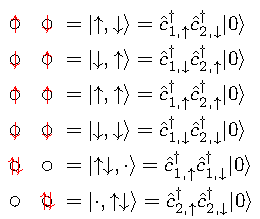
\includegraphics[scale=1]{2electronStates.pdf}
\end{figure}\\
And we have:
\begin{align}
\langle \uparrow,\downarrow|\uparrow\downarrow\rangle&=\langle 0|\hat{c}_{2,\downarrow}\hat{c}_{1,\uparrow}\hat{c}_{1,\uparrow}^\dagger\hat{c}_{2,\downarrow}^\dagger|0\rangle=\langle 0|(\mathbb{1}-\hat{c}_{1,\uparrow}^\dagger\hat{c}_{1,\uparrow})(\mathbb{1}-\hat{c}_{2,\downarrow}^\dagger\hat{c}_{2,\downarrow})|0\rangle=1\\
\langle \uparrow,\downarrow|\downarrow\uparrow\rangle&=\langle 0|\hat{c}_{2,\downarrow}\hat{c}_{1,\uparrow}\hat{c}_{1,\downarrow}^\dagger\hat{c}_{2,\downarrow}^\dagger|0\rangle=\langle 0|\hat{c}_{1,\downarrow}^\dagger\hat{c}_{2,\downarrow}^\dagger\hat{c}_{1,\uparrow}\hat{c}_{2,\downarrow}|0\rangle=\notag
\end{align}
Similar expressions can be obtain for all the other combinations of basis states. Using the anticommutation relations for the creation and annihilation operators we'd find that the states are orthonormal and basis states, shown below: are a basis of the Hilbert space. We can find the entries of the Hamiltonian matrix as follows:
\begin{equation}
H_{ij}=\langle i|\hat{H}|j\rangle
\end{equation}
Where $|i\rangle$ are the basis states. We can easily evaluate these expressions by first looking at which terms simply become zero because one or more creation or annihilation operators can be anticommutated to the left or right respectively to annihilate against the vacuum state $|0\rangle$.\\
\\
To save some work we can look at the three terms that make up the Hamiltonian individually and argue which entries will be non-zero. First we'll consider hopping term $\hat{H}_t$. Looking at our basis states we can see that hopping is only allowed for the states $|1\rangle,|2\rangle,|5\rangle$ and $|6\rangle$ and more specifically, the states with two occupied sites of opposite spin can hop into states with a single occupied state, also with opposite spin and vice versa.
\newpage
\noindent
The on-site interaction term $\hat{H}_U$ counts the products of the number of particles of opposite spin over the two sites. This term can thus only be non-zero if there is pair of opposite spins on a single site, thus only $|5\rangle$ and $|6\rangle$ will give non-zero diagonal contributions. The orbital energy term $\hat{H}_{\varepsilon_0}$ simply counts the electrons in each spin state at each site so all six states will have a non-zero diagonal contribution.\\
\\
So we have:
\begin{align}
\langle\uparrow,\downarrow|\hat{H}_t|\uparrow\downarrow,\cdot\rangle&=-t\langle0|\hat{c}_{2,\downarrow}\hat{c}_{1,\uparrow}(\hat{c}_{1,\uparrow}^\dagger \hat{c}_{2,\uparrow}+\hat{c}_{2,\uparrow}^\dagger \hat{c}_{1,\uparrow}+\hat{c}_{1,\downarrow}^\dagger \hat{c}_{2,\downarrow}+\hat{c}_{2,\downarrow}^\dagger \hat{c}_{1,\downarrow})\hat{c}_{1,\uparrow}^\dagger\hat{c}_{1\downarrow}^\dagger|0\rangle\\
&=-t\langle0|\hat{c}_{2,\downarrow}\hat{c}_{1,\uparrow}\hat{c}_{2,\downarrow}^\dagger \hat{c}_{1,\downarrow}\hat{c}_{1,\uparrow}^\dagger\hat{c}_{1\downarrow}^\dagger|0\rangle=-t\langle0|\hat{c}_{2,\uparrow}\hat{c}_{2,\uparrow}^\dagger \hat{c}_{1,\uparrow}\hat{c}_{1,\uparrow}^\dagger\hat{c}_{1,\downarrow}\hat{c}_{1\downarrow}^\dagger|0\rangle\notag\\
&=-t\notag\\
\langle\uparrow,\downarrow|\hat{H}_t|\cdot,\uparrow\downarrow\rangle&=-t\langle0|\hat{c}_{2,\downarrow}\hat{c}_{1,\uparrow}(\hat{c}_{1,\uparrow}^\dagger \hat{c}_{2,\uparrow}+\hat{c}_{2,\uparrow}^\dagger \hat{c}_{1,\uparrow}+\hat{c}_{1,\downarrow}^\dagger \hat{c}_{2,\downarrow}+\hat{c}_{2,\downarrow}^\dagger \hat{c}_{1,\downarrow})\hat{c}_{2,\uparrow}^\dagger\hat{c}_{2\downarrow}^\dagger|0\rangle\\
&=-t\langle0|\hat{c}_{2,\downarrow}\hat{c}_{1,\uparrow}\hat{c}_{1,\uparrow}^\dagger \hat{c}_{2,\uparrow}\hat{c}_{2,\uparrow}^\dagger\hat{c}_{2\downarrow}^\dagger|0\rangle=-t\langle0|\hat{c}_{1,\uparrow}\hat{c}_{1,\uparrow}^\dagger \hat{c}_{2,\uparrow}\hat{c}_{2,\uparrow}^\dagger\hat{c}_{2,\downarrow}\hat{c}_{2\downarrow}^\dagger|0\rangle\notag\\
&=-t\notag\\
\langle\downarrow,\uparrow|\hat{H}_t|\uparrow\downarrow,\cdot\rangle&=-t\langle0|\hat{c}_{2,\uparrow}\hat{c}_{1,\downarrow}(\hat{c}_{1,\uparrow}^\dagger \hat{c}_{2,\uparrow}+\hat{c}_{2,\uparrow}^\dagger \hat{c}_{1,\uparrow}+\hat{c}_{1,\downarrow}^\dagger \hat{c}_{2,\downarrow}+\hat{c}_{2,\downarrow}^\dagger \hat{c}_{1,\downarrow})\hat{c}_{1,\uparrow}^\dagger\hat{c}_{1\downarrow}^\dagger|0\rangle\\
&=-t\langle0|\hat{c}_{2,\uparrow}\hat{c}_{1,\downarrow}\hat{c}_{2,\uparrow}^\dagger \hat{c}_{1,\uparrow}\hat{c}_{1,\uparrow}^\dagger\hat{c}_{1\downarrow}^\dagger|0\rangle=t\langle0|\hat{c}_{2,\uparrow}\hat{c}_{2,\uparrow}^\dagger \hat{c}_{1,\uparrow}\hat{c}_{1,\uparrow}^\dagger\hat{c}_{1,\downarrow}\hat{c}_{1\downarrow}^\dagger|0\rangle\notag\\
&=t\notag\\
\langle\downarrow,\uparrow|\hat{H}_t|\cdot,\uparrow\downarrow\rangle&=-t\langle0|\hat{c}_{2,\uparrow}\hat{c}_{1,\downarrow}(\hat{c}_{1,\uparrow}^\dagger \hat{c}_{2,\uparrow}+\hat{c}_{2,\uparrow}^\dagger \hat{c}_{1,\uparrow}+\hat{c}_{1,\downarrow}^\dagger \hat{c}_{2,\downarrow}+\hat{c}_{2,\downarrow}^\dagger \hat{c}_{1,\downarrow})\hat{c}_{2,\uparrow}^\dagger\hat{c}_{2\downarrow}^\dagger|0\rangle\\
&=-t\langle0|\hat{c}_{2,\uparrow}\hat{c}_{1,\downarrow}\hat{c}_{1,\downarrow}^\dagger \hat{c}_{2,\downarrow}\hat{c}_{2,\uparrow}^\dagger\hat{c}_{2\downarrow}^\dagger|0\rangle=t\langle0|\hat{c}_{1,\uparrow}\hat{c}_{1,\uparrow}^\dagger \hat{c}_{2,\uparrow}\hat{c}_{2,\uparrow}^\dagger\hat{c}_{2,\downarrow}\hat{c}_{2\downarrow}^\dagger|0\rangle\notag\\
&=t\notag
\end{align}
And from these expressions we can also find the hermitian conjugates which are trivial when $t$ is real. We then have:
\begin{align}
\langle\uparrow\downarrow,\cdot|\hat{H}_U|\uparrow\downarrow,\cdot\rangle&=U\langle0|\hat{c}_{1,\downarrow}\hat{c}_{1,\uparrow}(\hat{c}_{1,\uparrow}^\dagger \hat{c}_{1,\uparrow}\hat{c}_{1,\downarrow}^\dagger \hat{c}_{1,\downarrow}+\hat{c}_{2,\uparrow}^\dagger \hat{c}_{2,\uparrow}\hat{c}_{2,\downarrow}^\dagger \hat{c}_{2,\downarrow})\hat{c}_{1,\uparrow}^\dagger\hat{c}_{1,\downarrow}^\dagger|0\rangle\\
&=U\langle0|\hat{c}_{1,\downarrow}\hat{c}_{1,\uparrow}\hat{c}_{1,\uparrow}^\dagger \hat{c}_{1,\uparrow}\hat{c}_{1,\downarrow}^\dagger \hat{c}_{1,\downarrow}\hat{c}_{1,\uparrow}^\dagger\hat{c}_{1,\downarrow}^\dagger|0\rangle\notag\\
&=U\langle0|\hat{c}_{1,\uparrow}\hat{c}_{1,\uparrow}^\dagger \hat{c}_{1,\downarrow}\hat{c}_{1,\downarrow}^\dagger \hat{c}_{1,\uparrow}\hat{c}_{1,\uparrow}^\dagger\hat{c}_{1,\downarrow}\hat{c}_{1,\downarrow}^\dagger|0\rangle\notag\\
&=U\notag\\
\langle \cdot,\uparrow\downarrow|\hat{H}_U|\cdot,\uparrow\downarrow\rangle&=U\langle0|\hat{c}_{2,\downarrow}\hat{c}_{2,\uparrow}(\hat{c}_{1,\uparrow}^\dagger \hat{c}_{1,\uparrow}\hat{c}_{1,\downarrow}^\dagger \hat{c}_{1,\downarrow}+\hat{c}_{2,\uparrow}^\dagger \hat{c}_{2,\uparrow}\hat{c}_{2,\downarrow}^\dagger \hat{c}_{2,\downarrow})\hat{c}_{2,\uparrow}^\dagger\hat{c}_{2,\downarrow}^\dagger|0\rangle\\
&=U\langle0|\hat{c}_{2,\downarrow}\hat{c}_{2,\uparrow}\hat{c}_{2,\uparrow}^\dagger \hat{c}_{2,\uparrow}\hat{c}_{2,\downarrow}^\dagger \hat{c}_{2,\downarrow}\hat{c}_{2,\uparrow}^\dagger\hat{c}_{2,\downarrow}^\dagger|0\rangle\notag\\
&=U\langle0|\hat{c}_{2,\uparrow}\hat{c}_{2,\uparrow}^\dagger \hat{c}_{2,\downarrow}\hat{c}_{2,\downarrow}^\dagger \hat{c}_{2,\uparrow}\hat{c}_{2,\uparrow}^\dagger\hat{c}_{2,\downarrow}\hat{c}_{2,\downarrow}^\dagger|0\rangle\notag\\
&=U\notag
\end{align}
Lastly for the orbital part of the Hamiltonian we get:
\begin{align}
\langle\uparrow\downarrow|\hat{H}_{\varepsilon_0}|\uparrow\downarrow\rangle&=\varepsilon_0\langle0|\hat{c}_{2,\downarrow}\hat{c}_{1,\uparrow}(\hat{c}_{1,\uparrow}^\dagger\hat{c}_{1,\uparrow}+\hat{c}_{1,\downarrow}^\dagger\hat{c}_{1,\downarrow}+\hat{c}_{2,\uparrow}^\dagger\hat{c}_{2,\uparrow}+\hat{c}_{2,\downarrow}^\dagger\hat{c}_{2,\downarrow})\hat{c}_{1,\uparrow}^\dagger\hat{c}_{2,\downarrow}^\dagger|0\rangle\\
&=\varepsilon_0\langle0|\hat{c}_{2,\downarrow}\hat{c}_{1,\uparrow}(\hat{c}_{1,\uparrow}^\dagger\hat{c}_{1,\uparrow}+\hat{c}_{2,\downarrow}^\dagger\hat{c}_{2,\downarrow})\hat{c}_{1,\uparrow}^\dagger\hat{c}_{2,\downarrow}^\dagger|0\rangle\notag\\
&=\varepsilon_0\langle0|\hat{c}_{1,\uparrow}\hat{c}_{1,\uparrow}^\dagger\hat{c}_{1,\uparrow}\hat{c}_{1,\uparrow}^\dagger\hat{c}_{2,\downarrow}\hat{c}_{2,\downarrow}^\dagger+\hat{c}_{1,\uparrow}\hat{c}_{2,\downarrow}^\dagger\hat{c}_{2,\downarrow}\hat{c}_{1,\uparrow}^\dagger\hat{c}_{2,\downarrow}\hat{c}_{2,\downarrow}^\dagger|0\rangle\notag\\
&=2\varepsilon_0\notag
\end{align}
The result is the same for all other states.
\newpage
\noindent
We can now explicitly write the Hamiltonian as a matrix for our chosen bases states:
\begin{equation}
H=\begin{pmatrix}
2\varepsilon_0 & 0 & 0 & 0 & -t & -t\\
0 & 2\varepsilon_0 & 0 & 0 & t & t\\
0& 0 & 2\varepsilon_0 & 0 & 0 & 0\\
0 & 0& 0 & 2\varepsilon_0 & 0 & 0\\
-t & t & 0& 0 & 2\varepsilon_0 + U & 0\\
-t & t & 0& 0&0 & 2\varepsilon_0+U\\
\end{pmatrix}
\end{equation}
Throwing this into Mathematica we can obtain the eigenvectors and corresponding eigenvalues:
\begin{align*}
|1\rangle&=|\!\uparrow,\uparrow\rangle\qquad\qquad&\hat{H}|1\rangle&=2\varepsilon_0|1\rangle\\
|2\rangle&=|\!\downarrow,\downarrow\rangle\qquad\qquad&\hat{H}|2\rangle&=2\varepsilon_0|2\rangle\\
|3\rangle&=\dfrac{1}{\sqrt{2}}(|\!\uparrow,\downarrow\rangle+|\!\downarrow,\uparrow\rangle)\qquad\qquad&\hat{H}|3\rangle&=2\varepsilon_0|3\rangle\\
|4\rangle&=\dfrac{1}{\sqrt{2}}(|\cdot,\uparrow\downarrow\rangle-|\uparrow\downarrow,\cdot\rangle)\qquad\qquad&\hat{H}|4\rangle&=(2\varepsilon_0+U)|4\rangle\\
|5\rangle&=\beta^-(\dfrac{4t}{\alpha-U}|\uparrow,\downarrow\rangle-\dfrac{4t}{\alpha-U}|\downarrow,\uparrow\rangle+|\uparrow\downarrow,\cdot\rangle+|\cdot\,\uparrow\downarrow\rangle)\qquad\qquad&\hat{H}|5\rangle&=(2\varepsilon_0+\dfrac{U-\alpha}{2})|5\rangle\\
|6\rangle&=\beta^+(\dfrac{-4t}{\alpha+U}|\uparrow,\downarrow\rangle+\dfrac{4t}{\alpha+U}|\downarrow,\uparrow\rangle+|\uparrow\downarrow,\cdot\rangle+|\cdot\,\uparrow\downarrow\rangle)\qquad\qquad&\hat{H}|6\rangle&=(2\varepsilon_0+\dfrac{U+\alpha}{2})|6\rangle
\end{align*}
Where
$$\alpha=\sqrt{16t^2+U}\qquad\beta^\pm=\dfrac{1}{\sqrt{2+32\bigg (\dfrac{t}{\alpha\pm U}\bigg )^2}}$$
For instead a single electron we only have the four basis states $|\uparrow,\cdot\rangle$, $|\downarrow,\cdot\rangle$, $|\cdot,\uparrow\rangle$ and $|\cdot,\downarrow\rangle$. It's clear by the above reasoning that we'd get the following Hamiltonian matrix:
\begin{equation}
H=\begin{pmatrix}
\varepsilon_0&0&-t&0\\
0&\varepsilon_0&0&-t\\
-t&0&\varepsilon_0&0\\
0&-t&0&\varepsilon_0
\end{pmatrix}
\end{equation}
With eigenvectors and corresponding eigenvalues:
\begin{align*}
|1\rangle&=\dfrac{1}{\sqrt{2}}(|\downarrow,\cdot\rangle+|\cdot,\downarrow\rangle)\qquad\qquad&\hat{H}|1\rangle&=(\varepsilon_0-t)|1\rangle\\
|2\rangle&=\dfrac{1}{\sqrt{2}}(|\uparrow,\cdot\rangle+|\cdot,\uparrow\rangle)\qquad\qquad&\hat{H}|2\rangle&=(\varepsilon_0-t)|2\rangle\\
|3\rangle&=\dfrac{1}{\sqrt{2}}(|\downarrow,\cdot\rangle-|\cdot,\downarrow\rangle)\qquad\qquad&\hat{H}|3\rangle&=(\varepsilon_0+t)|3\rangle\\
|4\rangle&=\dfrac{1}{\sqrt{2}}(|\uparrow,\cdot\rangle-|\cdot,\uparrow\rangle)\qquad\qquad&\hat{H}|4\rangle&=(\varepsilon_0+t)|4\rangle\\
\end{align*}
\newpage
\noindent
For the case of three electrons we have the following states: $|\!\uparrow,\uparrow\downarrow\rangle$, $|\!\downarrow,\uparrow\downarrow\rangle$, $|\!\uparrow\downarrow,\uparrow\rangle$ and $|\!\uparrow\downarrow,\downarrow\rangle$. Again, by the same reasoning we obtain the Hamiltonian:
\begin{equation}
H=\begin{pmatrix}
3\varepsilon_0+U&0&t&0\\
0&3\varepsilon_0+U&0&t\\
t&0&3\varepsilon_0+U&0\\
0&t&0&3\varepsilon_0+U
\end{pmatrix}
\end{equation}
With eigenvectors and corresponding eigenvalues:
\begin{align*}
|1\rangle&=\dfrac{1}{\sqrt{2}}(-|\downarrow,\uparrow\downarrow\rangle+|\uparrow\downarrow,\downarrow\rangle)\qquad\qquad&\hat{H}|1\rangle&=(3\varepsilon_0-t+U)|1\rangle\\
|2\rangle&=\dfrac{1}{\sqrt{2}}(-|\uparrow,\uparrow\downarrow\rangle+|\uparrow\downarrow,\uparrow\rangle)\qquad\qquad&\hat{H}|2\rangle&=(3\varepsilon_0-t+U)|2\rangle\\
|3\rangle&=\dfrac{1}{\sqrt{2}}(|\downarrow,\uparrow\downarrow\rangle+|\uparrow\downarrow,\downarrow\rangle)\qquad\qquad&\hat{H}|3\rangle&=(3\varepsilon_0+t+U)|3\rangle\\
|4\rangle&=\dfrac{1}{\sqrt{2}}(|\uparrow,\uparrow\downarrow\rangle+|\uparrow\downarrow,\uparrow\rangle)\qquad\qquad&\hat{H}|4\rangle&=(3\varepsilon_0+t+U)|4\rangle\\
\end{align*}
The Green function can be found using the Lehmann representation:
\begin{equation}
G_{\alpha,\beta}(i\omega_\nu)=\dfrac{1}{Z}\sum_{i,j}\dfrac{e^{-\beta(E_i-\mu N_i)}+e^{-\beta(E_j-\mu N_j)}}{i\omega_\nu+\mu-(E_j-E_i)}\langle i|\hat{c}_\alpha |j\rangle\langle j|\hat{c}_\beta^\dagger|i\rangle
\end{equation}
The operators $\hat{c}_\alpha$ and $\hat{c}_\beta^\dagger$ will decrease and increase the number of particles in the system, hence we needed to find the states for one and three electrons before we can find the Green Function for the system of two electrons. But I've encountered different notations for the Lehmann representation, namely:
\begin{equation}
G_{ij\sigma}(\omega)=\lim_{\eta\to 0^ +}\bigg (\sum_{m}\dfrac{\langle\Psi_0^N|\hat{c}_i|\Psi_m^ {N+1}\rangle\langle\Psi_m^ {N+1}|\hat{c}_j^\dagger|\Psi_0^ N\rangle}{\omega-(E_m^{N+1}-E_0^N)+i\eta}+\sum_{n}\dfrac{\langle\Psi_0^N|\hat{c}_j^\dagger|\Psi_n^ {N-1}\rangle\langle\Psi_n^ {N-1}|\hat{c}_i|\Psi_0^ N\rangle}{\omega-(E_n^{N+1}-E_0^N)+i\eta}\bigg )
\end{equation}
\newpage
\noindent
For the Hubbard Dimer with on-site Coulomb interactions with strength $U$ and long-range interactions with strength $V$ we have the following Hamiltonian:
\begin{align}
\hat{H}=&\ -t(\hat{c}_{1,\uparrow}^\dagger \hat{c}_{2,\uparrow}+\hat{c}_{2,\uparrow}^\dagger \hat{c}_{1,\uparrow}+\hat{c}_{1,\downarrow}^\dagger \hat{c}_{2,\downarrow}+\hat{c}_{2,\downarrow}^\dagger \hat{c}_{1,\downarrow}) + U(\hat{n}_{1,\uparrow}\hat{n}_{1,\downarrow}+\hat{n}_{2,\uparrow}\hat{n}_{2,\downarrow})\\
&+ V(\hat{n}_{1,\uparrow}\hat{n}_{2,\uparrow}+\hat{n}_{1,\uparrow}\hat{n}_{2,\downarrow}+\hat{n}_{1,\downarrow}\hat{n}_{2,\uparrow}+\hat{n}_{1,\downarrow}\hat{n}_{2,\downarrow})+ \varepsilon_0(\hat{n}_{1,\uparrow}+\hat{n}_{1,\downarrow}+\hat{n}_{2,\uparrow}+\hat{n}_{2,\downarrow})\notag
\end{align}
Using the same set of basis states we get the following Hamiltonian matrix:
\begin{equation}
H=\begin{pmatrix}
2\varepsilon_0+V & 0 & 0 & 0 & -t & -t\\
0 & 2\varepsilon_0+V & 0 & 0 & t & t\\
0& 0 & 2\varepsilon_0+V & 0 & 0 & 0\\
0 & 0& 0 & 2\varepsilon_0+V & 0 & 0\\
-t & t & 0& 0 & 2\varepsilon_0 + U & 0\\
-t & t & 0& 0&0 & 2\varepsilon_0+U\\
\end{pmatrix}
\end{equation}
\end{document}